% Created by tikzDevice version 0.12 on 2019-09-22 13:22:25
% !TEX encoding = UTF-8 Unicode
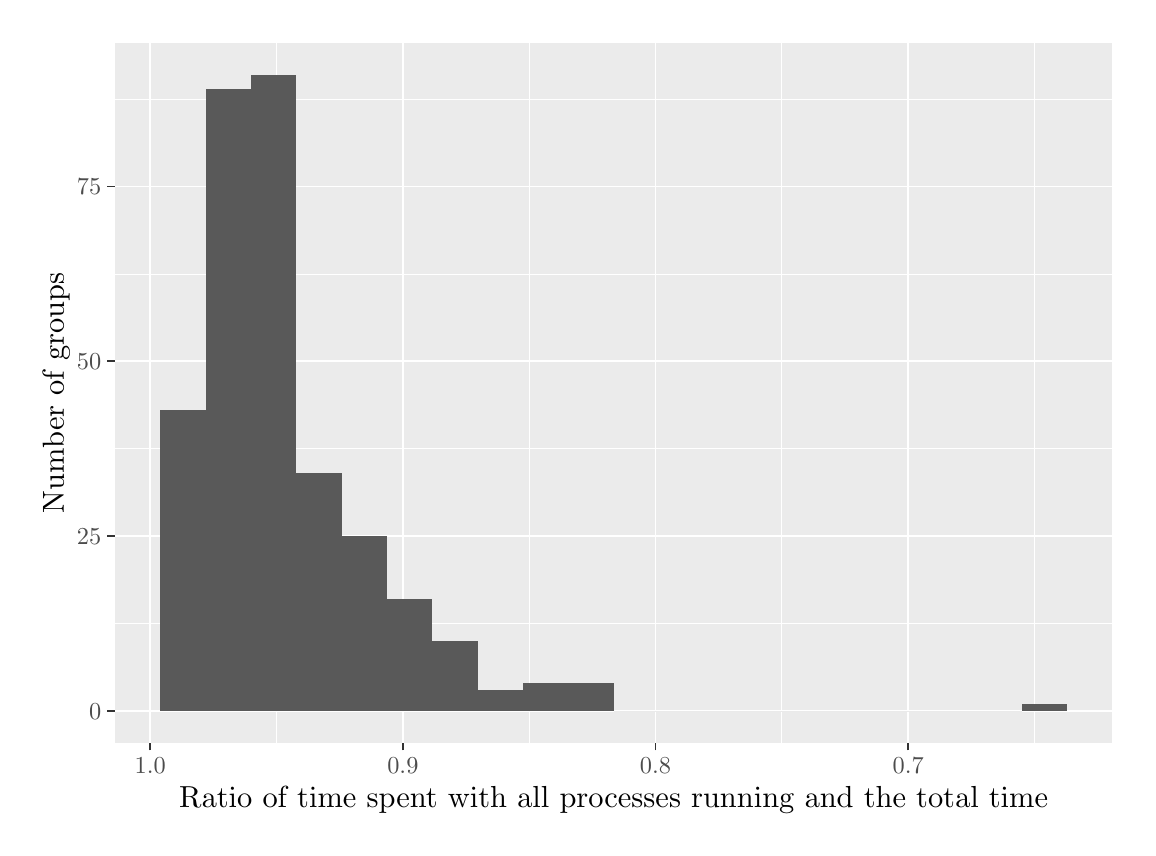
\begin{tikzpicture}[x=1pt,y=1pt]
\definecolor{fillColor}{RGB}{255,255,255}
\path[use as bounding box,fill=fillColor,fill opacity=0.00] (0,0) rectangle (397.48,289.08);
\begin{scope}
\path[clip] (  0.00,  0.00) rectangle (397.48,289.08);
\definecolor{drawColor}{RGB}{255,255,255}
\definecolor{fillColor}{RGB}{255,255,255}

\path[draw=drawColor,line width= 0.6pt,line join=round,line cap=round,fill=fillColor] (  0.00,  0.00) rectangle (397.48,289.08);
\end{scope}
\begin{scope}
\path[clip] ( 31.52, 30.72) rectangle (391.98,283.58);
\definecolor{fillColor}{gray}{0.92}

\path[fill=fillColor] ( 31.52, 30.72) rectangle (391.98,283.58);
\definecolor{drawColor}{RGB}{255,255,255}

\path[draw=drawColor,line width= 0.3pt,line join=round] ( 31.52, 73.79) --
	(391.98, 73.79);

\path[draw=drawColor,line width= 0.3pt,line join=round] ( 31.52,136.94) --
	(391.98,136.94);

\path[draw=drawColor,line width= 0.3pt,line join=round] ( 31.52,200.09) --
	(391.98,200.09);

\path[draw=drawColor,line width= 0.3pt,line join=round] ( 31.52,263.25) --
	(391.98,263.25);

\path[draw=drawColor,line width= 0.3pt,line join=round] (363.83, 30.72) --
	(363.83,283.58);

\path[draw=drawColor,line width= 0.3pt,line join=round] (272.53, 30.72) --
	(272.53,283.58);

\path[draw=drawColor,line width= 0.3pt,line join=round] (181.23, 30.72) --
	(181.23,283.58);

\path[draw=drawColor,line width= 0.3pt,line join=round] ( 89.93, 30.72) --
	( 89.93,283.58);

\path[draw=drawColor,line width= 0.6pt,line join=round] ( 31.52, 42.22) --
	(391.98, 42.22);

\path[draw=drawColor,line width= 0.6pt,line join=round] ( 31.52,105.37) --
	(391.98,105.37);

\path[draw=drawColor,line width= 0.6pt,line join=round] ( 31.52,168.52) --
	(391.98,168.52);

\path[draw=drawColor,line width= 0.6pt,line join=round] ( 31.52,231.67) --
	(391.98,231.67);

\path[draw=drawColor,line width= 0.6pt,line join=round] (318.18, 30.72) --
	(318.18,283.58);

\path[draw=drawColor,line width= 0.6pt,line join=round] (226.88, 30.72) --
	(226.88,283.58);

\path[draw=drawColor,line width= 0.6pt,line join=round] (135.58, 30.72) --
	(135.58,283.58);

\path[draw=drawColor,line width= 0.6pt,line join=round] ( 44.28, 30.72) --
	( 44.28,283.58);
\definecolor{fillColor}{gray}{0.35}

\path[fill=fillColor] ( 47.90, 42.22) rectangle ( 64.29,150.84);

\path[fill=fillColor] ( 64.29, 42.22) rectangle ( 80.67,267.03);

\path[fill=fillColor] ( 80.67, 42.22) rectangle ( 97.06,272.09);

\path[fill=fillColor] ( 97.06, 42.22) rectangle (113.44,128.10);

\path[fill=fillColor] (113.44, 42.22) rectangle (129.83,105.37);

\path[fill=fillColor] (129.83, 42.22) rectangle (146.21, 82.63);

\path[fill=fillColor] (146.21, 42.22) rectangle (162.60, 67.48);

\path[fill=fillColor] (162.60, 42.22) rectangle (178.98, 49.80);

\path[fill=fillColor] (178.98, 42.22) rectangle (195.37, 52.32);

\path[fill=fillColor] (195.37, 42.22) rectangle (211.75, 52.32);

\path[fill=fillColor] (211.75, 42.22) rectangle (228.14, 42.22);

\path[fill=fillColor] (228.14, 42.22) rectangle (244.52, 42.22);

\path[fill=fillColor] (244.52, 42.22) rectangle (260.91, 42.22);

\path[fill=fillColor] (260.91, 42.22) rectangle (277.29, 42.22);

\path[fill=fillColor] (277.29, 42.22) rectangle (293.68, 42.22);

\path[fill=fillColor] (293.68, 42.22) rectangle (310.06, 42.22);

\path[fill=fillColor] (310.06, 42.22) rectangle (326.45, 42.22);

\path[fill=fillColor] (326.45, 42.22) rectangle (342.83, 42.22);

\path[fill=fillColor] (342.83, 42.22) rectangle (359.22, 42.22);

\path[fill=fillColor] (359.22, 42.22) rectangle (375.60, 44.74);
\end{scope}
\begin{scope}
\path[clip] (  0.00,  0.00) rectangle (397.48,289.08);
\definecolor{drawColor}{gray}{0.30}

\node[text=drawColor,anchor=base east,inner sep=0pt, outer sep=0pt, scale=  0.88] at ( 26.57, 39.19) {0};

\node[text=drawColor,anchor=base east,inner sep=0pt, outer sep=0pt, scale=  0.88] at ( 26.57,102.34) {25};

\node[text=drawColor,anchor=base east,inner sep=0pt, outer sep=0pt, scale=  0.88] at ( 26.57,165.49) {50};

\node[text=drawColor,anchor=base east,inner sep=0pt, outer sep=0pt, scale=  0.88] at ( 26.57,228.64) {75};
\end{scope}
\begin{scope}
\path[clip] (  0.00,  0.00) rectangle (397.48,289.08);
\definecolor{drawColor}{gray}{0.20}

\path[draw=drawColor,line width= 0.6pt,line join=round] ( 28.77, 42.22) --
	( 31.52, 42.22);

\path[draw=drawColor,line width= 0.6pt,line join=round] ( 28.77,105.37) --
	( 31.52,105.37);

\path[draw=drawColor,line width= 0.6pt,line join=round] ( 28.77,168.52) --
	( 31.52,168.52);

\path[draw=drawColor,line width= 0.6pt,line join=round] ( 28.77,231.67) --
	( 31.52,231.67);
\end{scope}
\begin{scope}
\path[clip] (  0.00,  0.00) rectangle (397.48,289.08);
\definecolor{drawColor}{gray}{0.20}

\path[draw=drawColor,line width= 0.6pt,line join=round] (318.18, 27.97) --
	(318.18, 30.72);

\path[draw=drawColor,line width= 0.6pt,line join=round] (226.88, 27.97) --
	(226.88, 30.72);

\path[draw=drawColor,line width= 0.6pt,line join=round] (135.58, 27.97) --
	(135.58, 30.72);

\path[draw=drawColor,line width= 0.6pt,line join=round] ( 44.28, 27.97) --
	( 44.28, 30.72);
\end{scope}
\begin{scope}
\path[clip] (  0.00,  0.00) rectangle (397.48,289.08);
\definecolor{drawColor}{gray}{0.30}

\node[text=drawColor,anchor=base,inner sep=0pt, outer sep=0pt, scale=  0.88] at (318.18, 19.71) {0.7};

\node[text=drawColor,anchor=base,inner sep=0pt, outer sep=0pt, scale=  0.88] at (226.88, 19.71) {0.8};

\node[text=drawColor,anchor=base,inner sep=0pt, outer sep=0pt, scale=  0.88] at (135.58, 19.71) {0.9};

\node[text=drawColor,anchor=base,inner sep=0pt, outer sep=0pt, scale=  0.88] at ( 44.28, 19.71) {1.0};
\end{scope}
\begin{scope}
\path[clip] (  0.00,  0.00) rectangle (397.48,289.08);
\definecolor{drawColor}{RGB}{0,0,0}

\node[text=drawColor,anchor=base,inner sep=0pt, outer sep=0pt, scale=  1.10] at (211.75,  7.44) {Ratio of time spent with all processes running and the total time};
\end{scope}
\begin{scope}
\path[clip] (  0.00,  0.00) rectangle (397.48,289.08);
\definecolor{drawColor}{RGB}{0,0,0}

\node[text=drawColor,rotate= 90.00,anchor=base,inner sep=0pt, outer sep=0pt, scale=  1.10] at ( 13.08,157.15) {Number of groups};
\end{scope}
\end{tikzpicture}
